This section gives an overview of AGREE's assume-guarantee reasoning
system, abstractly defining the verification conditions that AGREE
checks in order to establish overall system correctness at the model
level.  The discussion then becomes more concrete, showing how the
AGREE contract specification language is used to specify the
cyber-hardened system of \figref{fig:hardened}. It explains the the
top-level specification of the example system, then shifts to the
specifications for the filter and the monitor.  These two
specifications are those that are synthesized to equivalent CakeML by
SPLAT.

%% These conditions are useful in understanding how the semantics in
%% synthesis differ from those in the assume-guarantee reasoning
%% in \secref{sec:semantics}.

\subsection{Verification conditions}

\newcommand{\globally}{\ensuremath{\mathbf{G}}}
\newcommand{\historically}{\ensuremath{\mathbf{H}}}
\newcommand{\assumes}{\ensuremath{A}}
\newcommand{\guarantees}{\ensuremath{P}}
\newcommand{\dispatch}{\ensuremath{\mathit{dispatch}}}
\newcommand{\complete}{\ensuremath{\mathit{complete}}}
\newcommand{\same}[1]{\ensuremath{\mathit{same}(#1)}}
\newcommand{\inputs}{\ensuremath{I}}
\newcommand{\outputs}{\ensuremath{O}}
\newcommand{\system}{\ensuremath{S}}
\newcommand{\components}{\ensuremath{C}}
\newcommand{\component}{\ensuremath{c}}
\newcommand{\schedule}{\ensuremath{\phi}}
\newcommand{\valid}{\ensuremath{\mathit{valid}}}
\newcommand{\dpred}{\ensuremath{\delta^\phi}}
\newcommand{\dispred}{\ensuremath{\mathbb{D}^\phi}}
\newcommand{\compred}{\ensuremath{\mathbb{C}^\phi}}
\newcommand{\dispredp}{\ensuremath{\mathbb{D}^{\phi\prime}}}
\newcommand{\compredp}{\ensuremath{\mathbb{C}^{\phi\prime}}}

The AGREE specification language is based on stream concepts, and
operators, from the Lustre language \cite{10.1145/41625.41641}. Thus
the setting is synchronous dataflow where the inputs and outputs of
components are streams, and contracts express relationships between
input and output streams. When considering a system of components,
data flows through the components in dependency order, with inputs
being propagated to outputs through all contracts until they stabilize
(can't propagate further). Therefore, the subcomponent contracts, and
thus the top-level model, must be acyclic. (An apparent syntactic
cycle, where a component is linked back to itself, may be broken
temporally by inserting delay elements.)  Once the data propagation
has stabilized, the model proceeds to the next input data in the input
streams. The semantics do not model computation or communication
delay. The output of one contract is seen at the input of any
downstream contract in the same step of the input data stream.

From the system and component contracts, AGREE generates a set of
verification conditions to show that a system's component
implementation is correct~\cite{agree2013}.  The AGREE model checker
is then invoked to prove or disprove the verification
conditions. Contracts and verification conditions are expressed in
\emph{past-time linear temporal logic} (PLTL).\footnote{KLS: citation
needed.}  PLTL is a logic enhanced with temporal operators able to
reason about the truth values of formulas through time.  Its semantics
are defined relative to a point in time $i$ and a finite trace of
system states $\pi = s_0, s_1, \ldots, s_i$.

The two PLTL operators necessary for the AGREE generated verification
conditions are $\globally$ (globally) that looks forward in time along
the trace and $\historically$ (historically) that looks backward in
time along the trace.  These are defined as
\begin{eqnarray*}
 (\pi, i) \models \globally(f) & \iff & \forall j \ge i, (\pi, j) \models f \\
(\pi, i) \models \historically(f) & \iff & \forall 0 \le j \le i, (\pi, j) \models f
\end{eqnarray*}
The $\models$-operator is read as \emph{satisfies}.  A trace at a
moment in time satisfies $\globally(f)$ if and only if it satisfies
$f$ in the current and all future states of $\pi$.  $\globally(f)$ is
invariant from the current moment into the future and $\historically$ is
invariant from the beginning of the trace to the current moment.

A \emph{system} $\system = (\inputs, \outputs, \assumes,
\guarantees,C)$, where $\inputs$ is the input set, $\outputs$ is the
output set, $\assumes$ is the set of assumptions, $\guarantees$ is the
set of guarantees, and $C$ are subcomponents.  A subcomponent
$\component$ is, hierarchically, also a system, and may be designated
by its own tuple $(\inputs_\component, \outputs_\component,
\assumes_\component, \guarantees_\component, C_c)$.  From the
components and their connections, $\mathbb{I}_\component$ is defined
to be the set of components providing input to some component
$\component$ in the system, and $\mathbb{O}$ is defined to be the set
of components that provide the output for the system.  A system $S$ is
\emph{correct} if and only if for all components $c \in C$ the
following two verification conditions hold:
\begin{equation}
            \globally(\historically(\assumes \wedge
            \bigwedge_{\component^\prime \in \mathbb{I}_\component} P_{\component^\prime})
            \implies \assumes_\component)
\end{equation}
\begin{equation}
            \globally(\historically(\assumes \wedge
            \bigwedge_{\component^\prime \in \mathbb{O}} \guarantees_{\component^\prime})
            \implies \guarantees)
\end{equation}
Condition (1) verifies the input assumptions on each component under
the system assumptions and upstream component guarantees.  It checks
if the component guarantees and system assumptions are strong enough
to imply input assumptions on all immediate downstream components.
Condition (2) checks the output guarantees of the system under the
system assumptions and component guarantees that provide the output.
It checks if the guarantees on components providing primary outputs
are strong enough to imply the system guarantees.

If all the verification conditions hold (AGREE uses $k$-inductive
model checking to automatically prove or disprove each generated
verification condition), then the system is said to be \emph{correct},
meaning that the system composition meets input assumptions at each
input as well as the guarantees on the system output. A consequence of
this result is that $\globally(\historically(\assumes) \implies
\guarantees)$ holds for the system contract.

The expanded property lists in \figref{fig:example-certificate} and
\figref{fig:hardened-certificate} are the results from verifying or
disproving the above verification conditions.  The additional
unexpanded results at the bottom of the figures prove
\emph{self-consistency} in the contracts.  It is not uncommon to
accidentally write contracts that are self-contradicting.  For
example, a contract may guarantee an output be two different values in
the same moment of time.  AGREE generates additional verification
conditions that prove each component contract, and the composition of
contracts, self-consistent.


\subsection{System contract}
\newsavebox{\sw}
\begin{lrbox}{\sw}
\begin{lstlisting}[style=agree,numbers=left]
eq req : bool = event(AutomationRequest);*\label{line:sw-event-def-start}*
eq avl : bool = event(AirVehicleLocation);
eq wp  : bool = event(Waypoint);
eq strt: bool = event(Start);
eq alrt: bool = event(Alert);*\label{line:sw-event-def-end}*

assume "Automation requests are well-formed" : *\label{line:sw-assume-1}*
  req => WELL_FORMED_AUTOMATION_REQUEST(AutomationRequest);
assume "Air vehicle locations are well-formed" : *\label{line:sw-assume-2}*
  avl => WELL_FORMED_WAYPOINT(AirVehicleLocation);
assume "One automation request in flight at a time" : *\label{line:sw-assume-3}*
  true ->
  (req => pre(Historically(not req) or Since(not req, strt)));

guarantee "Waypoints coincide with air vehicle locations": *\label{line:sw-guarantee-1}*
  wp => avl;
guarantee "Starts include a new waypoint" : *\label{line:sw-guarantee-2}*
  strt => wp;
guarantee "Waypoints are well-formed" :  *\label{line:sw-guarantee-3}*
  wp => WELL_FORMED_WAYPOINT(Waypoint);
guarantee "Starts within one cycle of requests if not alerting" : *\label{line:sw-guarantee-4}*
  (strt => ((not alrt) and req)) ->
  (strt => ((not alrt) and (req or pre(req))));
guarantee "Alert if not started within one cycle of requests" : *\label{line:sw-guarantee-5}*
  true -> ((pre(req and not strt) and not strt) => alrt);
guarantee "Once alerted always alerted" : *\label{line:sw-guarantee-6}*
  Once(alrt) => alrt;
\end{lstlisting}
\end{lrbox}

\begin{figure}
  \begin{center}
    \scalebox{0.62}{\usebox{\sw}}
  \end{center}
  \caption{The SW component contract.}
  \label{fig:sw}
\end{figure}

The actual surface syntax for AGREE that is embedded in OSATE is slightly different than the formal semantics in the previous section.
The mapping between the two is straightforward.
The AGREE specification for the SW component in the example of
Section~\ref{sec:example} is given in \figref{fig:sw}.  The
specification uses \texttt{eq} statements to define variables local to
the contract specification.  For
example, \lineref{line:sw-event-def-start} defines the \texttt{req}
variable to be equivalent to the \texttt{event} expression.

All the named ports in the corresponding AADL component are in the scope of the specification, and there are additional implicit boolean \emph{event} inputs (or outputs) associated with event ports.
An \texttt{event} expression refers to that implicit input (or output) boolean value and is true when data is present on the named port and false otherwise.
\linesref{line:sw-event-def-start}{line:sw-event-def-end} create local variables that are true when data is present on the corresponding event ports for the component.
The local variables here are purely for convenience in writing the specification.

The \texttt{assume} statement is a string description followed by a predicate.
Those on \lineref{line:sw-assume-1} and \lineref{line:sw-assume-2} are implications requiring that when data is present it is well-formed.
The well-formed predicates themselves are defined elsewhere using AGREE functions.

The assumption on \lineref{line:sw-assume-3} constrains when a request can arrive by reasoning about the \emph{state} of the contract.
The state of the contract is captured by stream semantics of AGREE.
When writing assumptions and guarantees, it is important to differentiate pre-state, before a contract updates its state, and post-state, after a contract updates its state, in response to the current input.
The \texttt{pre} naturally makes that distinction.
In general, assumptions regarding state should be evaluated in the pre-state of the component with the current inputs, and guarantees regarding state should be evaluated on the post-state of the component given the current inputs.
Guarantees should use \texttt{pre} anytime they need to reason about the current state relative to the previous state.

The assumption on \lineref{line:sw-assume-3} uses a followed-by expression so it is \texttt{true} at time 0 and then it is the truth value of the implication in all future instances.
The followed-by guards the \texttt{pre} as mentioned previously;
thus after time 0, the assumption depends on the presence of a request and the pre-state of the component.
The assumption on \lineref{line:sw-assume-3} is that if there is an incoming request, it is either the very first one, \texttt{\textbf{Historically}(\textbf{not} req)}, or it is after the component has output a start event in response to a previous request, \texttt{\textbf{Since}(\textbf{not} req, strt)}--\emph{not request since start}.

The guarantees on \linesref{line:sw-guarantee-1}{line:sw-guarantee-3} coincide events and assert well-formed output.
The guarantees on \linesref{line:sw-guarantee-4}{line:sw-guarantee-6} define temporal properties of the component.
\lineref{line:sw-guarantee-4} insists that a start happens with a request or one step after a request.
The guarantee uses the assumption on \lineref{line:sw-assume-3} and does not check for two requests in a row without a start as the assumption precludes that input behavior.
It differentiates with the followed-by what is required at time 0, the start must coincide with the request, with what is required after time 0, the start must coincide with the request or is a response to a request one step earlier.
The guarantee also does not force the start to always happen, it only says that if it does happen, it is under the defined conditions.

\lineref{line:sw-guarantee-5} forces the alert to sound if the start does not arrive within the one-step bound.
Together with \lineref{line:sw-guarantee-4} the contract model allows for non-alerting and alerting behavior.
\lineref{line:sw-guarantee-6} ensures if alert has ever happened, then it is happening in the present moment.
These six guarantees define the behavior of the SW component under the three assumptions and correspond to the informal descriptions given in \secref{sec:example}.

\subsection{Cyber-hardening the system implementation}
%% \begin{figure}
%%   \begin{center}
%%     \begin{tabular}{c}
%%     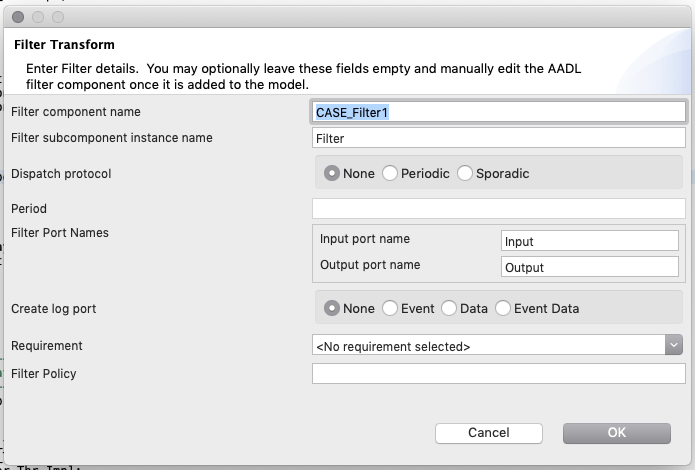
\includegraphics[scale=0.3]{dialogue.png}
%%     \end{tabular}
%%   \end{center}
%%   \caption{BriefCASE dialogue for filter transformation.}
%%   \label{fig:dialogue}
%% \end{figure}


Generally, AGREE contracts do not describe the computation that a
component performs. This is entirely by design: AGREE is intended to
reason about component behavior solely at the specification
level. However, the syntax of AGREE provides enough expressiveness to
support the notion of a \emph{code contract}: a contract from which an
implementation can be extracted. First we must discuss a class of
guarantees---\emph{output guarantees}---which determine the values on
all output ports of a component.

\begin{definition}[Output guarantee]
An \emph{output guarantee} is a stylized guarantee that fully
specifies the data written to an output port. There are three
possibilities according to whether the output port $p$ is
a \konst{data} port, an \konst{event} port, or an \konst{event data}
port:
\[
\begin{array}{ll}
\konst{data}: &  p = \mathit{e} \\
\konst{event}: &  \konst{event} (p) = \mathit{b} \\
\konst{event data}: & \itelse{b}{\konst{event} (p) \land p = e}{\neg \konst{event}(p)} \\
\end{array}
\]
\end{definition}

Informally, a code contract treats its \konst{eq} ``statements'' as
defining a list of assignments to state variables, and its output
guarantees as directives for producing output.

\begin{definition}[Code contract] A
  leaf component of the form $(I,O,A,P,\emptyset)$ is a
  \emph{code contract} if $\mathit{Eqs} \cup G \subseteq P$, where
\[\mathit{Eqs} = \set{v_1 = e_1, \cdots , v_n = e_n} \] is a non-empty set
of \konst{eq} statements and $G$ is the set of output guarantees, one for
each element of $O$. In the interpretation as code, the order of
elements of $\mathit{Eqs}$ is important, and is simply taken to be the
occurrence order of the \konst{eq} statements in the syntax. Thus we
will work with the
\emph{list} of equations $\mathit{Eqs} = [v_1 = e_1; \cdots ; v_n = e_n]$.
\end{definition}


The semantics of Section \ref{agree-semantics} supports a formal
connection between the original contract---and verification results of
the AGREE model checker being run on it---and code generated from
specifications of leaf level cyber-components. It also provides the
root meaning at the base of a chain of translation steps moving from
an AGREE contract to a CakeML executables.

The first step in the chain maps the contract to a code-focused
representation. Assume given a code contract
$(I,O,A,\mathit{Eqs} \cup G \cup P,\emptyset)$, environment $E$, and
time $t$. The \emph{evaluation} of $\mathit{Eqs}$ followed by the
evaluation of $G$ results in a new environment $E'$ where the stream
values for state variables and outputs have been computed for time
$t$. The step from $E$ to $E'$ is one full cycle in the repeated
evaluation of the component.

\begin{definition}[Evaluation]
We overload existing notation and write the evaluation of
$\mathit{Eqs}$ and then $G$ in environment $E$ at time $t$ as
$\sem{\mathit{Eqs}\cdot G}^E_t$. The evaluation of $v = e \in {\Eqs}$
is an environment transformation
\[
 \sem{v = e}^E_t = E[v(t) \mapsto\sem{e}^E_t] \ .
\]
modifying $E$ so that stream $v$ has value $\sem{e}^E_t$ at time $t$.
The list {\Eqs} is evaluated by folding the transformation left-to-right
through it. The transformation is similarly applied to the list of output
guarantees $G$, computing the values on output ports. The details are
omitted, being a bit messy because of the different kinds of output
ports available.
\end{definition}


\begin{definition}[Code contract correctness]
Assume code contract $(I,O,A,\mathit{Eqs} \cup G \cup P,\emptyset)$.
The contract is \emph{correct}, if for all $E$ and $t$, whenever the
assumptions (historically) hold in $E$ and evaluation steps from $E$
to $E'$, then the guarantees hold in $E'$:
\[
\sem{\konst{Hist}(A)}^E_t \land E' = \sem{\mathit{Eqs} \cdot G}^E_t \imp \sem{P}^{E'}_t
\]
\end{definition}
\footnote
{KLS: At this point we would like to assert that the AGREE ``consistency
 check'' for a contract implies code contract correctness.}

How does this notion of correctness integrate with the verification
conditions addressed by model checking? In \emph{contract
correctness}, the model checker is proving the following property
\[
\konst{Hist}(A) \imp P
\]
and in \emph{code contract correctness} we essentially prove a Hoare
triple of the form
\[
\set{\konst{Hist}(A)}\; (\mathit{Eqs} \cdot G) \; \set{P}
\]
This accords with intuition, namely that AGREE is a kind of
`program-free program logic'; by pulling out a program $(\mathit{Eqs}
\cdot G)$ from a code contract we find ourselves in the tepid
bathwater of imperative program verification. For example, at this
point one could apply a verification condition generator to help break
down the proof obligation. In order to use the code contract result in
system contract verifcation conditions, one has to show that the code
contract result implies the system verification condtion.

\subsubsection*{Wellformedness}
The evaluation semantics given above is based on the stream
computation model, where values arbitrarily `deep in the past' can be
accessed in computations by use of $\konst{pre}(-)$. However, the
conventional program languages we target do not support such a
view. We are currently examining transformations that compile such
deep temporal accesses away by introducing intermediate
variables. Avoiding discussion of the algorithm, we focus on the
notion of \emph{wellformed} equations that needs to hold. The guiding
intuition is that an \emph{implementable} {\Eqs} can allow access at
most one step in the past, and accesses of a past value for a variable
are only possible until the variable is updated. In lieu of a formal
definition, we give a few examples.

\begin{definition}[Wellformedness]

\end{definition}

\subsection{Code contracts for the hardened system}

\newsavebox{\flt}
\begin{lrbox}{\flt}
  \begin{lstlisting}[style=agree,numbers=left]
    -- start user definitions
    eq policy : bool =
      WELL_FORMED_AUTOMATION_RESPONSE(Input);
    -- stop user definitions

    guarantee "Filter output is well-formed" :
      if event(Input) and policy then
        event(Output) and Output = Input
      else
        not event(Output);
  \end{lstlisting}
\end{lrbox}

\newsavebox{\mntr}
\begin{lrbox}{\mntr}
  \begin{lstlisting}[style=agree,numbers=left]
    const is_latched : bool = true;

    -- start user definitions
    assume "One automation request in flight at a time" : *\label{line:mon-assume}*
      true -> (req => pre(Historically(not req) or Since(not req, rsp)));

    const MAX_LATENCY : int = 1; *\label{line:mon-const}*

    eq rsp : bool = event(Response);
    eq req : bool = event(Request);

    eq isPending : bool = Since(not rsp, req and not rsp);*\label{line:mon-pending}*
    eq latency : int = 0 -> (if req then 0 else pre(latency) + 1);*\label{line:mon-latency}*

    eq policy : bool = (rsp => req) ->
                         (    (isPending => latency < MAX_LATENCY)
                          and (rsp => (req or pre(isPending))));
    *\label{line:mon-policy}*
    -- stop user definitions

    eq alert : bool = (not policy) -> *\label{line:mon-alert}*
                        ((is_latched and pre(alert)) or not policy);

    guarantee "Alert port tracks alert variable" :
      event(Alert) = alert;
    guarantee "Output if not alerted" :
      if (not(alert) and rsp) then
          event(Output) and (Output = Response)
      else
          not (event(Output));
  \end{lstlisting}
\end{lrbox}

\begin{figure}
  \begin{center}
    \begin{tabular}{c}
      \scalebox{0.62}{\usebox{\flt}} \\
    \end{tabular}
  \end{center}
  \caption{Code contract specification for high-assurance filter.}
  \label{fig:filter}
\end{figure}

\begin{figure}
  \begin{center}
    \begin{tabular}{c}
    \scalebox{0.62}{\usebox{\mntr}} \\
    \end{tabular}
  \end{center}
  \caption{Code contract specification for high-assurance monitor.}
  \label{fig:monitor}
\end{figure}


As previously discussed, transformations carried out in the BriefCASE
interface have created a cyber-hardened system, protecting against
malicious AI behavior, by inserting a high-assurance filter and
monitor between the AI and the WM (see \figref{fig:hardened}). The
filter protects the WM from malformed data and the monitor protects
the WM from (possibly malicious) spontaneous or delayed responses.
These components were added, one at a time, by
\begin{enumerate}
  \item selecting the connection in the model where the
    component is to appear,
  \item choosing the appropriate transformation, and
  \item specifying the relevant filtering or monitoring \emph{policy} (behavior).
\end{enumerate}

%% The system designer provides configuration parameters for the
%% transformation in a dialogue box.  The dialogue box for adding a
%% filter is shown in \figref{fig:dialogue}.  All high-assurance
%% components rely on a \emph{policy} to define behavior as seen in the
%% last field of the dialogue box.  A filter policy defines well-formed
%% data while a monitor policy defines an invariant over inputs and
%% outputs.  These policies can be stated directly in the wizard, or they
%% can be left blank and added later to the AGREE contract generated by
%% the transformation.

BriefCASE creates all the needed AADL for the new high-assurance
component, and its connections in the system implementation, as part
of the transformation.  It also creates a default AGREE specification
that defines everything about the component behavior, leaving only the
component behavior (policy) to be specified.


Code contracts for the filter and monitor are shown in
\figref{fig:filter} and \figref{fig:monitor}.\footnote{KLS: do we discuss wellformedness anywhere?} In general, the
\konst{eq}-statements of a code contract keep track of
state and provide data values from which to compute values to place on
the outputs.

\subsubsection{Monitor specification}
BriefCASE generates everything but the
\konst{eq}-statements in \linesref{line:mon-assume}{line:mon-policy} of
\figref{fig:monitor}.  As with the filter, the guarantees
completely define the output, as required for synthesis, in terms of
the policy and the alert.  The
\texttt{alert} variable defined on \lineref{line:mon-alert} depends
not just on the policy but also on configuration details supplied when
the component is specified.  At configuration
time, \texttt{is\_latched} has been set to \konst{true}, thus making
the alert persistent, meaning that once the alert is raised, it is
always raised; otherwise, it is the complement of the policy value in
the current step.

The monitor policy is defined by marking when a request is not
satisfied, \texttt{isPending} on \lineref{line:mon-pending}, and
counting the number of steps between requests, \texttt{latency} on
\lineref{line:mon-latency}.  The \texttt{isPending} variable is true
whenever there is a request that does not coincide with a
response--\emph{not response since request and not response}.  The
\texttt{latency} variable starts at zero, resets on every request, and
otherwise increments by one.

The latency bound for the monitor is defined by the constant
\texttt{MAX\_LATENCY} on \lineref{line:mon-const}.  Here the constant
is set to one to be consistent with the system specification from the
previous section.  At time 0 the policy is trivial: a response
requires an accompanying request.  After time 0, if a request is
pending in the current time step, then the latency must still be under
the bound, and if there is a response, then it closes a request now or
a pending request from earlier in time.

The policy definition only works if there is never more than one
outstanding request at a time; otherwise, the latency counter resets
incorrectly.  That requirement is encoded in the assumption on
\lineref{line:mon-assume} and is the same assumption used for the
system input.  The policy can be written without needing the
assumption, but it is much simpler to write with the assumption.

As shown in \figref{fig:hardened-certificate}, the cyber-hardened
system passes AGREE verification.  That means that the high-assurance
components protect the WM from the untrusted AI generating malformed
data, spontaneous responses, or delayed responses.  Synthesis must
generate precise implementations of the high-assurance component
specifications for the AGREE verification result to apply to the
deployed system.  Precise in this context means that the
implementations match the input to output relations defined in the
specifications.

